\documentclass{article}
\usepackage[utf8x]{inputenc}
\usepackage{ucs}
\usepackage{amsmath} 
\usepackage{amsfonts}
\usepackage{marvosym}
\usepackage{wasysym}
\usepackage{upgreek}
\usepackage[english,russian]{babel}
\usepackage{graphicx}
\usepackage{float}
\usepackage{textcomp}
\usepackage{hyperref}
\usepackage{geometry}
  \geometry{left=2cm}
  \geometry{right=1.5cm}
  \geometry{top=1cm}
  \geometry{bottom=2cm}
\usepackage{tikz}
\usepackage{ccaption}
\usepackage{multicol}

\hypersetup{
   colorlinks=true,
   citecolor=blue,
   linkcolor=black,
   urlcolor=blue
}

\usepackage{listings}
%\setlength{\columnsep}{1.5cm}
%\setlength{\columnseprule}{0.2pt}

\usepackage[absolute]{textpos}


\usepackage{colortbl,graphicx,tikz}
\definecolor{X}{rgb}{.5,.5,.5}

\renewcommand{\thesubsection}{\arabic{subsection}}

\begin{document}
\pagenumbering{gobble}
\lstset{
  language=C++,
  basicstyle=\linespread{1.1}\ttfamily,
  columns=fixed,
  fontadjust=true,
  basewidth=0.5em,
  keywordstyle=\color{blue}\bfseries,
  commentstyle=\color{gray},
  stringstyle=\ttfamily\color{orange!50!black},
  showstringspaces=false,
  numbersep=5pt,
  numberstyle=\tiny\color{black},
  numberfirstline=true,
  stepnumber=1,
  numbersep=10pt,
  backgroundcolor=\color{white},
  showstringspaces=false,
  captionpos=b,
  breaklines=true,
  breakatwhitespace=true,
  xleftmargin=.2in,
  extendedchars=\true,
  keepspaces = true,
}

\lstset{ literate={~}{{\raisebox{0.5ex}{\texttildelow}}}{1} }
\newcommand\upquote[1]{\textquotesingle#1\textquotesingle}

\renewcommand{\thesubsection}{\arabic{subsection}}
\makeatletter
\def\@seccntformat#1{\@ifundefined{#1@cntformat}%
   {\csname the#1\endcsname\quad}%    default
   {\csname #1@cntformat\endcsname}}% enable individual control
\newcommand\section@cntformat{}     % section level 
\newcommand\subsection@cntformat{Задача \thesubsection.\space} % subsection level
\newcommand\subsubsection@cntformat{\thesubsubsection.\space} % subsubsection level
\makeatother


\makeatletter
\newcount\my@repeat@count
\newcommand{\myrepeat}[2]{%
  \begingroup
  \my@repeat@count=\z@
  \@whilenum\my@repeat@count<#1\do{#2\advance\my@repeat@count\@ne}%
  \endgroup
}
\makeatother

\title{Семинар \#8: Умные указатели. Домашнее задание.\vspace{-5ex}}\date{}\maketitle


\subsection{test}
\begin{lstlisting}
#include <iostream>
#include <memory>

struct Cat
{
    Cat() {std::cout << "Constructor" << std::endl;}
    ~Cat() {std::cout << "Destructor" << std::endl;}
};

int main()
{
    Cat* raw = new Cat;
    std::unique_ptr<Cat> p(raw);
    std::unique_ptr<Cat> q(raw);
}
\end{lstlisting}


\subsection{Односвязный список, используя \texttt{std::unique\_ptr}}
Создайте шаблонный класс \texttt{ForwardList<T>}, при этом, поле в узле списка, которое будет указывать на следующий узел должно иметь тип \texttt{std::unique\_ptr}. Поля такого класса должны выглядеть так:

\begin{lstlisting}
template <typename T>
class ForwardList
{
    struct Node
    {
        T value;
        std::unique_ptr<Node> next;
    };
    
    std::unique_ptr<Node> mpHead;
    Node* mpTail;
	...
};
\end{lstlisting}

Схематическое строение объекта такого класса:

\begin{center}
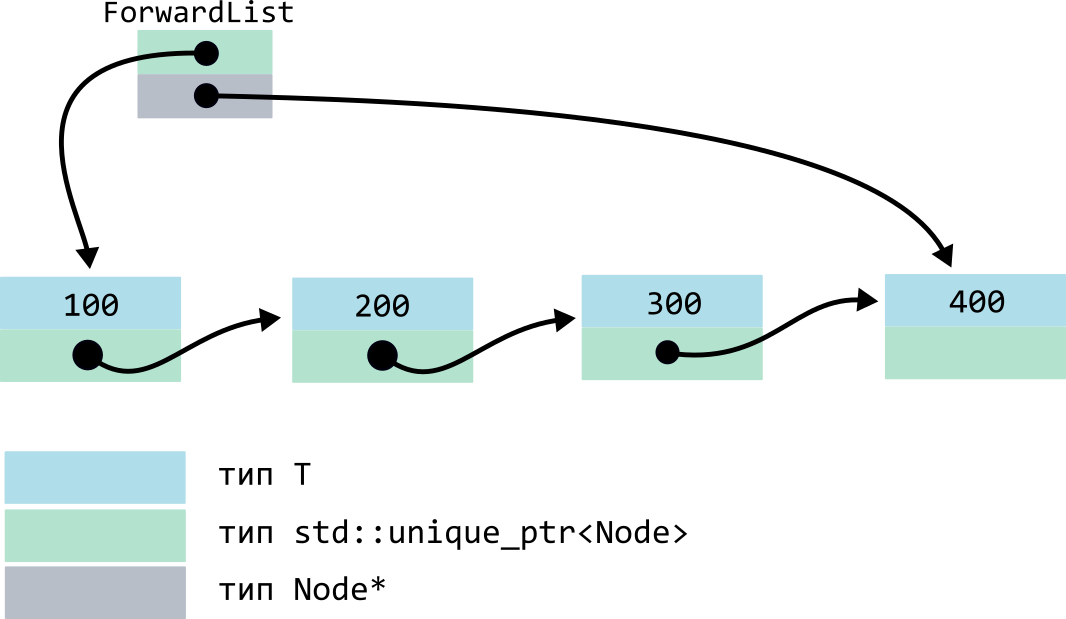
\includegraphics[scale=1]{../images/forward_list_unique.png}
\end{center}

Вам нужно написать следующие методы данного класса:

\begin{itemize}
\item Конструктор по умолчанию.
\item \texttt{void print()}
\item \texttt{void push\_front(T elem)}
\item \texttt{void push\_back(T elem)}
\item \texttt{std::unique\_ptr<T> pop\_front()}
\item \texttt{std::unique\_ptr<T> pop\_back()}
\item \texttt{void clear()}
\item \texttt{template <typename F> void foreach(F f)} -- применяет функцию \texttt{f} к каждому элементу связного списка. Функция f должна принимать объект типа \texttt{T} по обычной ссылке.


\item \texttt{void swap(ForwardList\& fl)} - меняет местами содержимое данного связного списка и списка \texttt{fl}.
\item \texttt{ForwardList copy()} - возвращает полную копию данного связного списка.
\end{itemize}


\end{document}
